\section{Reverse}
\subsection{Implementazione}
Per invertire la lista basta invertire i puntatori PAHEAD e PBACK di ogni 
nodo e impostare il puntatore al primo elemento della lista con l'indirizzo 
dell'ultimo elemento. Come mostrato in Figura~\ref{fig:reverse}

\begin{figure}[h]
    \centering
    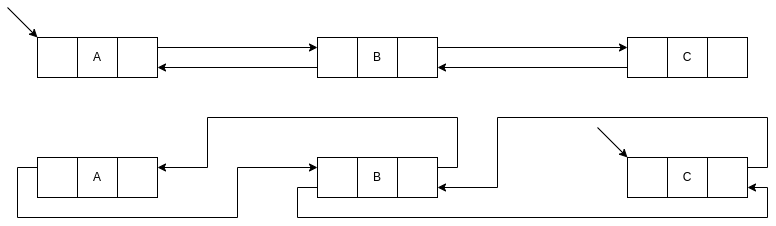
\includegraphics[scale=0.4]{diagrams/reverse.png}
    \caption{Rappresentazione lista prima e dopo reverse}
    \label{fig:reverse}
\end{figure}